%\documentclass[12pt,a4paper]{report}
\documentclass[12pt,a4paper,oneside,onecolumn,openright]{book}
% set the document language
\usepackage[italian]{babel}
% set the encoding used by your editor here (default is utf8)
\usepackage[utf8]{inputenc}
\usepackage[T1]{fontenc}

% math packages
\usepackage{amsmath}
\usepackage{amssymb}
\usepackage{lmodern}
\usepackage{varwidth}
\usepackage{xcolor}
\usepackage[makeroom]{cancel}
% page margins settings
\usepackage[inner=1.5cm,outer=1.5cm,top=1.5cm,bottom=1.5cm]{geometry}
%\usepackage{indentfirst}

% other packages
\usepackage{array}
\usepackage{enumitem}
\usepackage{subfigure}
\usepackage{graphicx}
\usepackage{verbatim}
\usepackage{listings}
\usepackage{url}
\usepackage[hidelinks]{hyperref}
\usepackage[export]{adjustbox}
\usepackage{latexsym}
\usepackage{tabularx}
\usepackage{ragged2e}
\usepackage{mathtools}
\DeclarePairedDelimiter\floor{\lfloor}{\rfloor}
\DeclarePairedDelimiter\ceil{\lceil}{\rceil}
% \usepackage{Mathematics}
% custom colors
\usepackage{color}
\usepackage{wrapfig}
\usepackage{gensymb}
\usepackage{caption}
\usepackage{tikz}
\usetikzlibrary{arrows.meta, positioning}
\usepackage{forest}
\usepackage{tikz-qtree}

\newcommand\myeq{\stackrel{\mathclap{\tiny\mbox{def}}}{=}}

\usepackage[many]{tcolorbox}
\newtcolorbox{boxA}{
    % fontupper = \bf,
    boxrule = 1.5pt,
    colframe = black % frame color
}

\usetikzlibrary{shadows}
\definecolor{light-gray}{gray}{0.96}
\definecolor{cyan}{RGB}{230,230,255}
\definecolor{dkgreen}{rgb}{0,0.6,0}
\definecolor{gray}{rgb}{0.5,0.5,0.5}
\definecolor{mauve}{rgb}{0.58,0,0.82}
\definecolor{iceberg}{rgb}{0.44, 0.65, 0.82}
% \definecolor{blue}{RGB}{44, 44, 210}

\hypersetup{
colorlinks=true,
linkcolor=black,
% filecolor=blue,
urlcolor=blue,
% pdftitle={Overleaf Example},
}

\urlstyle{same}
\graphicspath{ {./images/} }

% environment for bash code
\lstset{ %
  language=bash,                % the language of the code
  basicstyle=\footnotesize,           % the size of the fonts that are used for the code
  numbers=left,                   % where to put the line-numbers
  numberstyle=\footnotesize,          % the size of the fonts that are used for the line-numbers
  stepnumber=1,                   % the step between two line-numbers. If it's 1, each line 
                                  % will be numbered
  numbersep=5pt,                  % how far the line-numbers are from the code
  backgroundcolor=\color{white},      % choose the background color. You must add \usepackage{color}
  showspaces=false,               % show spaces adding particular underscores
  showstringspaces=false,         % underline spaces within strings
  showtabs=false,                 % show tabs within strings adding particular underscores
%  frame=single,                   % adds a frame around the code
  rulecolor=\color{black},        % if not set, the frame-color may be changed on line-breaks within not-black text (e.g. commens (green here))
  tabsize=2,                      % sets default tabsize to 2 spaces
  captionpos=b,                   % sets the caption-position to bottom
  breaklines=true,                % sets automatic line breaking
  breakatwhitespace=false,        % sets if automatic breaks should only happen at whitespace
  title=\lstname,                   % show the filename of files included with \lstinputlisting;
                                  % also try caption instead of title
  numberstyle=\tiny\color{gray},        % line number style
  keywordstyle=\textbf,          % keyword style
  commentstyle=\color{dkgreen},       % comment style
%  stringstyle=\color{mauve},         % string literal style
  escapeinside={\%*}{*)},            % if you want to add a comment within your code
  morekeywords={*,...,insert,-}               % if you want to add more keywords to the setù
}

% environment for python code
\lstset{
	language=Python,
	breaklines=true,
	breakatwhitespace=true ,
	backgroundcolor=\color{light-gray}
}

\newcommand{\grayScale}{0.95} % Can change the gray level here
\definecolor{codeBackground}{rgb}{\grayScale ,\grayScale ,\grayScale}
\definecolor{forestGreen}{rgb}{0.13,0.55,0.13}

\lstset{
    language=C,
    backgroundcolor=\color{codeBackground},
    tabsize=4,
    showstringspaces=false,
    showtabs=false,
    showspaces=false,
    basicstyle=\ttfamily,
    identifierstyle=\ttfamily,
    keywordstyle=\color{blue},
    stringstyle=\color{red},
    commentstyle=\color{gray},
    numberstyle=\color{magenta},
    morecomment=[l][\color{forestGreen}]{\#},
    % escapechar={|}, 
}
% appendices package
%\usepackage{appendix}
% set Appendix name used in the toc
%\renewcommand{\appendixtocname}{Appendice}

% interline
\linespread{1.5}
% set numbers for subsections and show them in the toc
\setcounter{tocdepth}{3} 
\setcounter{secnumdepth}{3}

% layout package, style and settings
\usepackage{fancyhdr}
\pagestyle{fancy}

\fancypagestyle{mainmatter}{%		
		\fancyhf{} 
		\fancyhead{}
		\fancyhead[LE,RO]{\thepage}
		\fancyhead[LO]{\footnotesize{\leftmark}}
		\fancyhead[RE]{\footnotesize{\rightmark}}
		\fancyfoot{}
		\addtolength{\headwidth}{\marginparsep}
		\addtolength{\headheight}{2.5pt}
		\renewcommand{\headrulewidth}{0.3pt}
		\renewcommand{\footrulewidth}{0.0pt}
		}
\fancypagestyle{frontmatter}{%
		\fancyhf{} 
		\fancyhead[LE]{\footnotesize{\MakeUppercase{\thepage}}}
		\fancyhead[RO]{\footnotesize{\MakeUppercase{\thepage}}}
		\fancyhead[RE,LO]{}
		\fancyfoot{}
		\addtolength{\headwidth}{\marginparsep}
		\addtolength{\headheight}{2.5pt}
		\renewcommand{\headrulewidth}{0.0pt}
		\renewcommand{\footrulewidth}{0.0pt}
		}
		
		
\usepackage{fancyhdr}
\pagestyle{fancy}
		\fancyhf{} 
		\fancyhead{}
		\fancyhead[LE,RO]{\thepage} 
		\fancyhead[LO]{\footnotesize{\leftmark}}
		\fancyhead[RE]{\footnotesize{\rightmark}}
		\fancyfoot{}
		\addtolength{\headwidth}{\marginparsep}
		\addtolength{\headheight}{2.5pt}
		\renewcommand{\headrulewidth}{0.3pt}
		\renewcommand{\footrulewidth}{0.0pt}

% empty pages have no numbers
\makeatletter
\def\cleardoublepage{\clearpage\if@twoside \ifodd\c@page\else
\hbox{}
  %Potresti voler togliere il commento dalla linea seguente
  %Questa pagina � stata lasciata intenzionalmente vuota.
\thispagestyle{empty}
\newpage
\if@twocolumn\hbox{}\newpage\fi\fi\fi}
\makeatother
%????
%\textwidth=450pt\oddsidemargin=0pt

%\makeatletter 
%  \DeclareRobustCommand*\textsubscript[1]{% 
%    \@textsubscript{\selectfont#1}} 
%  \newcommand{\@textsubscript}[1]{% 
%    {\m@th\ensuremath{_{\mbox{\fontsize\sf@size\z@#1}}}}} 
\makeatother 

\begin{document}
\begin{titlepage}
\begin{center}
{
    \large
    \textbf{Università  degli studi di Modena e Reggio Emilia} \\
   	\textbf{Dipartimento di Ingegneria Enzo Ferrari} \\
    \vspace{\stretch{0.5}}
    \hspace*{0cm} \hrulefill \hspace*{0cm} \\
    \vspace{\stretch{0.5}}    
	  \vspace{\stretch{12}}
  
  
 		\huge{\bf Crittografia Applicata }}\\
		\vspace{3mm}
		
		\vspace{\stretch{6}}
		\end{center}
		
\vspace{40mm}
\par
\noindent
\vspace{20mm}
\begin{center}
\hspace*{0cm} \hrulefill \hspace*{0cm} \\
{\large{\bf 
Anno Accademico 2023/24}}
\end{center}

\end{titlepage}

\pagestyle{frontmatter}
\frontmatter

% PAGINA VUOTA
%\clearpage\null\thispagestyle{empty}\clearpage
\setcounter{tocdepth}{2}
\tableofcontents

\setlength{\parindent}{12pt}
\setlength{\parskip}{1ex plus 0.5ex minus 0.2ex}
\mainmatter
\pagestyle{mainmatter}

\chapter{Introduction}

\section{Structure and Content}
\begin{itemize}

    \item \textbf{Module 1}: 
    \begin{enumerate}
        \item \textbf{\textit{intra-vehicles communications}}: nodes, sensors, ECU
        \item \textbf{\textit{signal busses}}: CAN, LIN, FlexRay, MOST, Ethernet [ T1/T1S]
        \item \textbf{\textit{car domain and OS}}
    \end{enumerate}
    
    \item \textbf{Module 2}:
    \begin{enumerate}
        \item \textbf{\textit{inter-vehicles communications}}: \textit{V2V} and \textit{V2X} (car is a node)
        \item \textbf{\textit{wireless technologies}}: Bluetooth, LoRa, C-V2X, IEE 802.11p (bd)
        \item application, messages, broadcast, GPS
    \end{enumerate}

\end{itemize}
Different \textbf{domain} or \textbf{application} needs different \textit{communications protocols}, is important to understand how each nodes in domain communicate each other (inside the car).

\newpage
\section{Intra-Vehicles}
From the 80's, where the car's control unit are isolated an there was a dedicated wires connect sensors and actuators with less electronic than now, until the reach the greates goal of evolution in the automotive sector: autonomous drive. The complexity of the number of connection from each ECU's to the other, also the number of ECU's for each car, is growing. While the number of signal increase in a liner way, the connection between ECU's is growing with a quadratic complexity $O(n^2)$.

If we examine the evolutions of the ECUs number inside an ``Audi A6'' we can observe that in 1997 it has 5 ECUs and in the 2007 it has 50 ECUs, instead the ``Tesla M3'' in the 2017 has 70 ECUs. The quadratic increase of ECUs number, however has reach a cap for two main reason: the cost and the space inside the car. Traditionally one ECUs is responsible of one task, but nowadays it could be two type of trends:
\begin{enumerate}[nosep]
    \item \textit{distributed of function across ECUs}
    \item \textit{integration of multiple function in one ECU}
\end{enumerate}

\section{Architectures}

\begin{figure}[h]
    \centering
    \begin{minipage}[t]{0.45\textwidth}
        \centering
        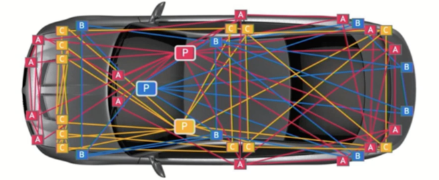
\includegraphics[width=\textwidth]{img/domain_architecture}
        \caption{\textit{Domain Architecture}}
        
        \begin{flushleft}
            \begin{enumerate}[nosep]
                \item central domain controller (\textbf{P}) or high performance computer
                \item ability to handle more complex functions
                \item cost optimization
                \item cable harness is rigid and expensive
            \end{enumerate}
        \end{flushleft}

    \end{minipage}
    \begin{minipage}[t]{0.45\textwidth}
        \centering
        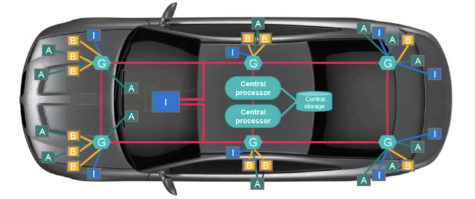
\includegraphics[width=\textwidth]{img/zonal_architecture}
        \caption{\textit{Zonal Architecture}}
        
        \begin{flushleft}
            \begin{enumerate}[nosep]
                \item local ethernet per zone (\textbf{G})
                \item ultra high-speed secured backbone between zone
                \item centralized software
                \item central computer storage
            \end{enumerate}
        \end{flushleft}
        
    \end{minipage}
\end{figure}
\chapter{Crittografia Simmetrica}

\begin{figure}[h]
    \centering
    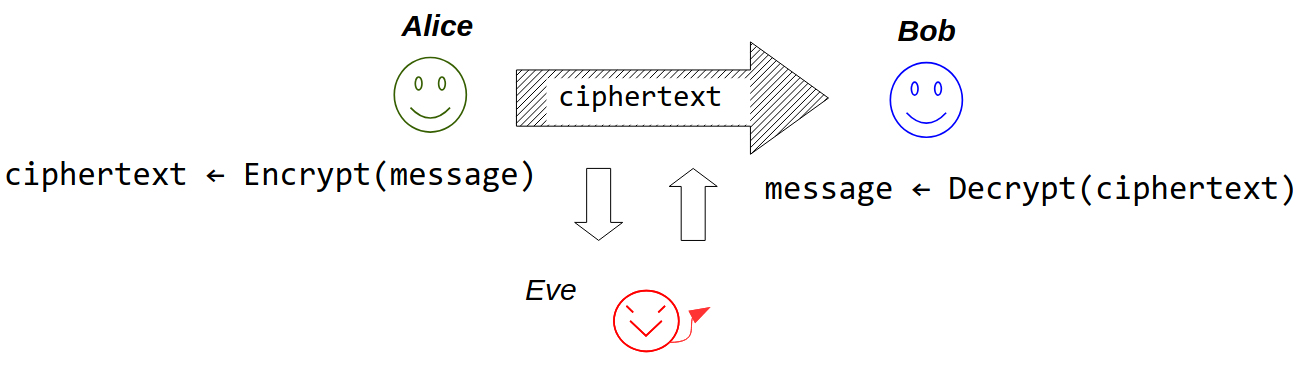
\includegraphics[width=\textwidth]{img/crypto_symm_1.png}
\end{figure}

Le garanzie di sicurezze che si cercano di mantenere sono:
\begin{itemize}[nosep]
    \item \textbf{confidenzialità}: Eve non può accedere a nessuna della informazioni sul messaggio.
    \item \textbf{autenticazione}: Bob può verificare se il messaggio non è stato inviato da Alice, viene anche chiamata \textbf{\textit{data orgin authenticity}} nel contesto della comunicazioni e implica anche la protezione contro modifiche illegittime (\textbf{integrità}).
\end{itemize}

\begin{flushleft}
    La sicurezza non esiste in natura è quindi necessario idearla e modellarla, questa prima parte prende il nome di \textit{Definitional Activity}. È comunque importante ricordare che le \textbf{definizioni} possono essere \textbf{errate} principalmente per errori nella modellazione o nello sviluppo software, ma anche perché non si è stato in grado di modellare quello che era invece richiesto. Un altro errore che si può essere portati a fare è quello di utilizzare in maniera errata certe definizioni ad esempio al di fuori del contesto per cui era stata definita. \newline
    \textbf{\textit{Definitional Activity}}: permette di descrivere che cosa l'avversario può \textbf{fare} e cosa può \textbf{vedere}. Esistono molteplici modi per definire la sicurezza in maniera più formale, uno tra questi è la \textbf{\textit{simulation-based security}} dove viene definita una funzione ideale che soddisfa la definizione di security e poi dimostrare che la funzione costruita si comporti come quella ideale.
\end{flushleft}

\begin{figure}[h]
    \centering
    \begin{large}
        \textbf{\textit{First Adversary Model}} \\
    \end{large}
    Quindi modelliamo e identifichiamo le casistiche e tipologie di un attaccante. \\

    \begin{minipage}[t]{0.50\textwidth}
        \centering
        \begin{boxA}
            \textcolor{red}{\textbf{\textit{Attack Model: Passive Eavesdropper (EAV)}}} \\
            Ha capacità di lettura dei soli \textit{ciphertext} e non è capace di \textbf{scegliere nulla}
        \end{boxA}
    \end{minipage}
    \begin{minipage}[t]{0.45\textwidth}
        \centering
        \begin{boxA}
            \textcolor{red}{\textbf{\textit{Security Goal: Indistinguishably}}} \\
            L'avversario non può distinguere il \textit{ciphertext} da sequenza di caratteri random.
        \end{boxA}
    \end{minipage}
\end{figure}

\begin{flushleft}
    Modellando in questo modo il nostro avversario è possibile osservare che non viene descritto nulla sul nascondere la lunghezza del \textit{plaintext}, infatti per questa prima modellazione l'avversario può vedere la lunghezza del \textit{plaintext}. \\
    \textbf{Nota}: la crittografia non ha come obiettivo quello di nascondere la lunghezza del testo in chiaro, nel caso in cui questa informazione fosse confidenziale, è necessario proteggerla a livello applicativo.
\end{flushleft}

\begin{flushleft}
    Le capacità di un avversario vengono espresse e descritte tramite degli algoritmi chiamati \textbf{esperimenti}, che vengono eseguiti da un'entità chiamata \textbf{\textit{challenger}} (che per semplicità andiamo ad identificare nell'attore onesto). \\
    Come prima andiamo ad analizzare \textbf{\textit{IND-EAV}}, il \textit{challenger} va a scegliere un messaggio \textbf{m} che viene scelto con la stessa probabilità tra:
    \begin{itemize}[nosep]
        \item dati random: $m \leftarrow \{0, 1\}^n$
        \item un messaggio generato attraverso la cifrazione $m = \text{Encryption}(p)$, dove \textbf{p} può essere scelto nello stesso modo di prima $p \leftarrow \{0, 1\}^n$
    \end{itemize}
    All'avversario viene fornito \textbf{m} e deve scegliere se è un messaggio randomico o se è l'output dell'\textit{encryption}, l'avversario vince l'esperimento se la sua decisione è corretta.
\end{flushleft}

\begin{flushleft}
    \textcolor{red}{\textbf{\textit{IND-EAV: Perfect \& Computational Indistinguishably}}} \\
    Andremo a discutere due tipologie di sicurezza:
    \begin{enumerate}[nosep]
        \item \textbf{\textit{perfect}}: la probabilità dell'avversario di vincere l'esperimento è del \textbf{50\%}, viene anche chiamata \textbf{\textit{Unconditional Security}} o \textbf{\textit{Informatition Theoretic Security}}.
        \item \textbf{\textit{computational}}: la probabilità dell'avversario di vincere l'esperimento è \textbf{50\%} più una \textbf{quantità trascurabile}.
    \end{enumerate}
    Qualunque tipologia di schema \textbf{praticabile} garantisce \textbf{sicurezza computazionale}, e se capace di essere sicuro contro un'\textbf{esperimento IND-EAV} viene detto \textbf{\textit{IND-EAV secure}}.
\end{flushleft}

\section{Sicurezza Incondizionata \& One-Time Pad}
\textcolor{red}{\textbf{XOR}}: gli schemi di crittografia moderni sono progettati per \textbf{dati binari}. L'operazione base per la crittografia simmetrica è lo \textbf{XOR}.

\begin{center}
    \begin{minipage}[c]{0.3\textwidth}
        \centering
        $c = m \oplus k$
    \end{minipage}
    \begin{minipage}[c]{0.3\textwidth}
        \centering
        \begin{tabular}{|c|c|c|}
            \hline
            \textbf{m} & \textbf{k} & \textbf{c} \\ \hline
            0 & 0 & 0 \\ \hline
            0 & 1 & 1 \\ \hline
            1 & 0 & 1 \\ \hline
            1 & 1 & 0 \\ \hline
        \end{tabular}
    \end{minipage}
    \begin{minipage}[c]{0.3\textwidth}
        \centering
        \textbf{Nota}: lo \textbf{XOR} può essere anche modellato come la somma bit per bit modulo 2: $c_i = (m_i \oplus k_i) \; \text{mod} \; 2$
    \end{minipage}
\end{center}

\begin{flushleft}
    Lo XOR viene scelto perché dato un certo \textbf{m}, se \textbf{k} viene scelta in maniera randomica la probabilità di \textbf{c} di essere \textbf{0} o \textbf{1} è \textbf{p = 0.5}. \\
    In questo modo sapere \textbf{c} non da informazioni su \textbf{m} e quindi \textbf{c} è indistinguibile da una successioni di bit random: $\{0, 1\}^n$
\end{flushleft}

\begin{flushleft}
    \textcolor{red}{\textbf{\textit{One-Time Pad - Vernam's Cipher}}}: è un algoritmo di crittografia che esegue un XOR bit a bit tra il testo in chiaro e la chiave, le due lunghezze devono essere uguali e la chiave devere essere random. $c_i = m_i \oplus k_i \; \forall i \in \{0, ..., n\}$ dove $n$ è la lunghezza del testo in chiaro. \\
    Per la decifrazione bisogna utilizzare la stessa chiave: $m = c \oplus k = (m \oplus k) \oplus k = m \oplus (k \oplus k) = m$. \\
    Anche se \textbf{OTP} è \textbf{incondizionatamente sicuro} non è praticabile realmente in quanto la generazione della chiave per testo arbitrario è computazionalmente onerosa ed è un algoritmo completamente \textbf{malleabile}. Gli schemi di crittografia oggi usati sono \textbf{computazionalmente sicuri}.
\end{flushleft}

\begin{flushleft}
    \textcolor{red}{\textbf{Nota sulla randomicità in crittografia}}: la randomicità in crittografia è differente da quella ``statistica'', ovvero una \textbf{distribuzione uniforme di 0 e 1} (che è necessaria ma non sufficiente), ma deve essere \textbf{\textit{unpredictable}}, in modo tale che anche osservando una sequenza, più o meno lunga di bit, non sia possibile predirre il bit successivo.
\end{flushleft}

\section{Sicurezza Computazionale: Security Level e Key Sizes}
Gli schemi crittografici moderni hanno come parte dei requisiti i \textbf{\textit{Kerckhoffs principle}} e necessitano uno \textbf{spazio delle chiavi largo} abbastanza per prevenire attacchi di ricerca esaustiva. Inoltre lo schema deve essere progettato in modo che si possa prevenire crittanalisi sul crittogramma, quindi nessuna informazione deve essere ottenuta dal crittogramma indipendentemente dal tipo di dato e deve essere sicura contro l'esperimento IND-EAV. 

Le condizioni necessarie avere degli schemi computazionalmente sicuri sono:
\begin{itemize}[nosep]
    \item gli schemi utilizzati devono essere computazionalmente sicuri.
    \item definiamo $F_k$ come una \textbf{PRF - \textit{Pseudo-Random Function}} con una chiave fissa \textbf{k} scelta randomicamente.
    \begin{itemize}[nosep]
        \item la \textbf{chiave} deve essere ``\textbf{corta}'' (ma lunga abbastanza per resistere ad attacchi a forza bruta).
        \item deve essere capace di cifrare grandi moli di dati.
        \item data la \textbf{chiave} le funzioni di \textbf{\textit{encryption}} e \textbf{\textit{decryption}} devono essere \textbf{efficenti}.
        \item senza la \textbf{chiave} la probabilità di rompere lo schema crittografico deve essere \textbf{trascurabile}.
    \end{itemize}
\end{itemize}

\begin{flushleft}
    È necessario tradurre in termini algoritmici \textbf{efficenti} e \textbf{trascurabile}. Alice e Bob che usano la funzione di \textit{encryption} e \textit{decryption} con la chiave devono essere capaci di eseguire gli algoritmi con costo \textit{efficient}, quindi il \textbf{costo computazionale} e \textbf{di memorizzazione} sono \textbf{polinomiali} sui parametri di sicurezza. Eve, che non conosce la chiave deve operare in maniera attraverso algoritmi \textbf{inefficienti}. \\
    $\rightarrow$ se il costo dell'attacco diverge da quello degli attori legittimi, è possibile scegliere i parametri di sicurezza appropriati in modo tale che la probabilità di completare correttamente l'algoritmo si molto piccola: \textbf{trascurabile}. 
\end{flushleft}

\begin{flushleft}
    Se fissiamo come probabilità di successo per definire un attacco a \textit{brute force} \textbf{inefficiente} $10^{-6}$, identifichiamo il valore di \textbf{N} per funzioni che hanno costo computazionale diverso, per quali valori di \textbf{n > N} le probabilità di sucesso sono inferiori?

    \begin{center}
        \begin{tabular}{lllll}
            \textbf{Costo di Esecuzione} && \textbf{Probabilità di Successo} && \textbf{\textit{Threshold}, b = 2} \\
            $\mathbf{O}(b^n)$ & $\rightarrow$ & $\mathbf{O}(b^{-n})$ & $\rightarrow$ & \textbf{N = 20} \\
            $\mathbf{O}(b^{\sqrt{n}})$ & $\rightarrow$ & $\mathbf{O}(b^{- \sqrt{n}})$ & $\rightarrow$ & \textbf{N = 400} \\
            $\mathbf{O}(b^{\log n})$ & $\rightarrow$ & $\mathbf{O}(b^{- \log n})$ & $\rightarrow$ & \textbf{N = 32}
        \end{tabular}
    \end{center}
    La conoscenza del costo dell'attacco più noto determina il valore del parametro di sicurezza, tra gli altri, la \textbf{dimensione della chiave}, identificato dal valore \textbf{N}.

    {\centering
        $\exists N \; | \; f(n) < \frac{1}{p(n)}, \; \forall n < N$
    \par}
\end{flushleft}

\begin{boxA}
    \textcolor{orange}{\textbf{Esempio}} \\
    Definiamo il costo di cifrazione $c_{enc}(n) = n$ mentre il costo dell'attacco $c_{attack} = n^2$ dove $n$ è la lunghezza della chiave. \\
    Negli anni 2000 l'\textit{encryption} utilizzava una chiave a 64bit e impiegava 1ms, mentre l'attacco a forza bruta, impiegava 2 anni. Dopo 10 anni, nel 2010, con la stessa chiave la cifrazione impiegava 0.1ms e il suo brute force 2 mesi. \\ \newline
    Aumentando la lunghezza della chiave, raddoppiandola, la fase di cifrazione impiegava 0.2ms, mentre quella di \textit{brute force} passava da $2^{64}$ a $2^{128} \simeq 10^{20}$ mesi.
\end{boxA}

\begin{flushleft}
    Grazie a nuove scoperte vengono trovati algoritmi che \textbf{indeboliscono} o \textbf{compromettono} il cifrario. Ad esempio alcuni schemi vengono pubblicamente violati pochi anni dopo la loro scoperta come gli schemi crittografici della famiglia \textit{rc} o \textit{sha1}. È anche possibile che schemi standard vengano indeboliti attraverso \textit{backdoor}, parametri deboli o ``particolari'' e implementazioni deboli.
\end{flushleft}

\begin{flushleft}
    \textcolor{red}{\textbf{\textit{Efficient function}}} $\rightarrow$ \textbf{\textit{polynomial}} \\
    Il costo (computazionale e memorizzativo) sono polinomiali rispetto ad un certo parametro di sicurezza $n$, algoritmi di \textit{encryption} costano al massimo: 
    
    {\centering
        $p(n) := a \cdot n^x$
    \par}

    \textcolor{red}{\textbf{\textit{Negligible function}}} $\rightarrow$ \textbf{\textit{smaller that any inverse polynomial}} \\
    Esiste un valore di \textbf{N} tale che la funzione sia minore di qualsialsi funzione polinomiale:

    {\centering
        $\exists N \; \text{t.c.} \; f(n) < \frac{1}{p(n)}, \; \forall \; n < N$
    \par}
\end{flushleft}

\begin{flushleft}
    \textcolor{red}{\textbf{\textit{PseudoRandom functions}}} \\
    Definiamo una \textbf{funzione ideale} che soddisfa computazionalmente l'esperimento di sicurezza IND-EAV, nel caso di crittografia a chiave privata, questo tipo di funzione si chiama \textbf{\textit{(keyed) family of PseudoRandom Function (PRF)}}.

    {\centering
        $\mathbf{F} \; : \; \mathbf{K} \times \mathbf{P} \mapsto \mathbf{C}$
    \par}

    Dove:
    \begin{itemize}[nosep]
        \item \textbf{K} è uniformemente scelto da $\{0, 1\}^{Lk(n)}$
        \item \textbf{P} è il \textit{plaintext} scelto arbitrariamente da $\{0,1\}^{Lp(n)}$
        \item \textbf{C} soddisfa computazionalmente \textbf{IND-EAV}, dove la ``quantità trascurabile'' è espressa dalla funzione \textbf{negl(n)} 
    \end{itemize}

    Uno schema di crittografia deve essere \textbf{funzionale}. Definiamo \textbf{F} come la \textbf{PRF} allora \textbf{F} si definirà computazionalmente sicura se:
    \begin{itemize}[nosep]
        \item lo spazio della chiavi è ``\textbf{piccolo}'', ma grande a sufficienza per resistere ad attacchi basati su ricerca esaustiva. Quindi $Lk(n)$ \textbf{deve} essere una funzione efficiente.
        \item ha la capacità di generare in output grande quantità di dati \textbf{\textit{pseudorandom}} (è sicuro per IND-EAV).
        \item il costo di computazione di \textbf{F} è \textbf{efficiente}.
        \item senza la chiave, la probabilità di rompere lo schema crittografico è \textbf{trascurabile}, il costo di calcolare $\mathbf{F}^{-1}$ è \textbf{inefficiente}.
    \end{itemize}
\end{flushleft}

\begin{flushleft}
    \textcolor{red}{\textbf{\textit{Concrete parameters for acceptable security guarantees}}} \\
    Gli schemi di crittografia (simmetrica) moderni vengono considerati computazionalmente sicuri, tali schema possono essere violati se si dispone di abbastanza tempo e abbastanza risorse. \\
    Il \textbf{\textit{Security Level}} dello schema è la media del numero di operazioni necessarie per rompere lo schema: gli standard stabiliscono dei valori tali che la quantità di tempo e risorse necessaria per calcolare tale quantità di operazioni è \textit{unfeasible}.
    \begin{itemize}[nosep]
        \item 80-bit di sicurezza $\rightarrow \; 2^{80}$ operazioni in media per rompere lo schema (insicuro dal 2010).
        \item 112-bit di sicurezza $\rightarrow \; 2^{112}$ operazioni in media per rompere lo schema (insicuro dal 2030).
        \item 128-bit di sicurezza $\rightarrow \; 2^{128}$ operazioni in media per rompere lo schema (stimata la sicurezza per ogni scenario successivo).
    \end{itemize}

    Nei moderni \textbf{schemi di crittografia simmetrica}, la \textbf{lunghezza della chiave} definisce il \textbf{livello di sicurezza}, in quanto l'attacco \textit{best-known} è basato sull'indovinare il segreto. A differenza, negli \textbf{schemi di crittografia asimmetrica} dove invece è presente solo una correlazione, in quanto dipende dagli attacchi noti alla matematica sottostante. \\

    Software e librerie \textbf{dovrebbero} implementare configurazioni \textbf{sicure} di \textbf{default} e aggiornate se necessarie
\end{flushleft}

\begin{flushleft}
    \textcolor{red}{\textbf{\textit{Asymmetric Cryptography \& Quantum Computers (PQC)}}} \\
    Si stima che gli attuali standard di crittografia asimmetrica saranno efficacemente violati dai computer quantistici nei prossimi decenni. Nell'ultimo decennio, sono stati ipotizzati e analizzati a fondo nuovi problemi cosiddetti ``\textbf{\textit{post-quantum hard problems}}'', ovvero che non possono essere risolti in modo efficiente nemmeno con un computer quantistico.
\end{flushleft}

\section{Stream Cipher}
\chapter{Hash Function \& MAC}

\begin{flushleft}
    Abbiamo visto che le configurazioni di sicurezza della crittografia simmetrica sono: \textbf{confidenzialità}, \textbf{integrità} e \textbf{autenticità}. Abbiamo anche definito che Alice e Bob condividono la conoscenza di un'unica chiave per la comunicazione. Con i \textit{block cipher} siamo riusciti a ottenere \textbf{confidenzialità}. 

    \medskip

    \textcolor{red}{\textbf{\textit{Integrity}}}: è possibili identificare dal ricevente di un messaggio se quel messaggio è stato modificato durante la trasmissione. Consideriamo una comunicazione tra Alice e Bob, dove il messaggio verrà inviato da Alice, prima di farlo verrà calcolato a \textbf{\textit{small-sized digest}} che rappresenta il dato. In questo modo qualunque modifica al dato o al \textbf{\textit{digest}} può essere verificata - in questo caso non c'è bisogno della chiave - $d = H(m)$ dove:
    \begin{itemize}[nosep]
        \item \textbf{d} è il \textit{digest} della funzione.
        \item \textbf{H} è una funziona che ritorna una sequenza di byte che rappresenta il dato.
        \item \textbf{m} è il messaggio.
    \end{itemize}
    Alice a quel punto invia a Bob $m || d$ in questo modo, Bob può ricalcolarsi $d' = H(m)$ e accettare il messaggio da Alice - quindi verificarne l'\textbf{integrità} - se e solo se $d == d'$.

    \medskip

    \textcolor{red}{\textbf{\textit{Authenticity Guarantess}}}: il destinatario del messaggio può controllare se il mittente è un mittente legittimo - ovvero qualcuno che ha accesso alla chiave segreta simmetrica - è possibile \textit{bindare} una qualche informazione (metadato) per rendere l'informazione identificativa, ma quasto è utile solamente nella crittografia asimmetrica.

    \begin{figure}[h]
        \centering
        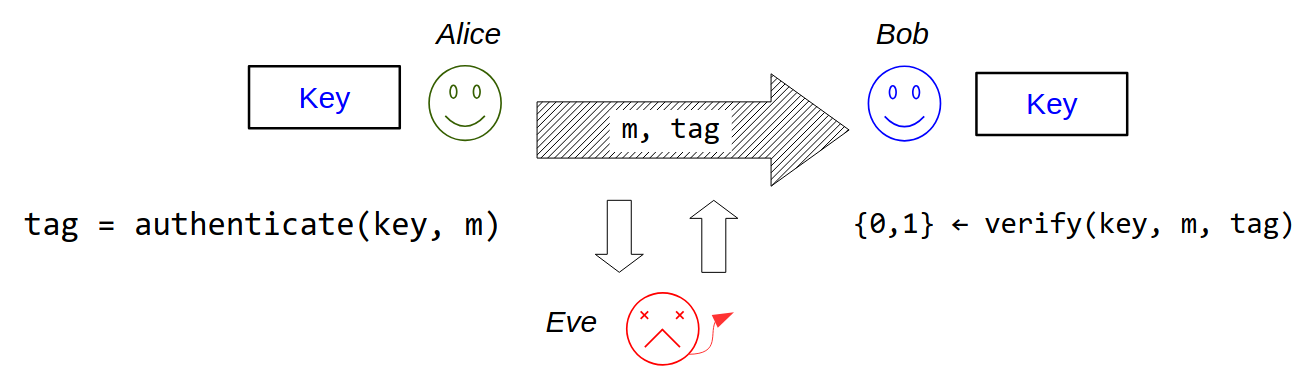
\includegraphics[width=0.55\textwidth]{img/mac_tag.png}
    \end{figure}

    L'integrità dell'informazione è condizione necessaria per l'autenticità, se l'attaccante può modificare il dato, allora può anche impersonificare il mittente del dato, violando l'autenticità.

    \smallskip

    È spesso confusa l'integrità del dato con la sua autenticità, nel contesto della sicurezza informatica noi cerchiamo l'autenticità - e quindi implicitamente l'integrità - per questo motivo andremo ad analizzare \textbf{\textit{authenticated encryption}}. È però fondamentale differenziare le due proprietà in quanto utilizzano schemi di crittografia differenti:
    \begin{itemize}[nosep]
        \item \textbf{\textit{Integrity}} utilizzo delle \textbf{funzioni hash}.
        \item \textbf{\textit{Authenticity}} utilizza i \textbf{\textit{Message Authentication Code - MAC}}, per ora andremo ad analizzarli nell'ambito della crittografia simmetrica.
    \end{itemize}

    \textcolor{red}{\textbf{\textit{Hash function \& cryptographic integrity guarantees}}} \\
    Andiamo, velocemente, ad analizzare quelle situazioni in cui è richiesta \textbf{\textit{integrità}} fuori dai requisiti di crittografia: come ad esempio modifiche al dato per errori di trasmissione o per guasti - normalmente scaturite da fenomeni fisici - per i quali sono presenti molteplici algoritmi, tra i quali: \textbf{\textit{parity}}, \textbf{CRC}, \textbf{\textit{checksum}}. In questo caso è possibile modellare la tipologia di attaccante come un \textbf{attaccante irrazionale} (perdita di bit randomici o a raffica). \\
    Nei settaggi di crittografia moderna, l'attaccante è sempre \textbf{razionale} e conosce gli \textbf{algoritmi crittografici} e si comporta di conseguenza, grazie al requisito di \textbf{\textit{cryptographic integrity-protection}} anche se noti i dati di base non deve essere capace di trovare una soluzione al problema nonostante l'assenza di una chiave condivisa. Anche in questo caso è presente la sicurezza computazione ma viene applicata in maniera differente.

\end{flushleft}

\section{Hash Function}

\begin{flushleft}

    \textcolor{red}{\textbf{Cryptography Hash Function}}: una funzione hash $H$ viene definita come: 

    {\centering
        $H : \{0, 1\}^* \mapsto \{0, 1\}^n$
    \par}

    ovvero è possibile mappare una quantità arbitraria di bit - nelle moderne funzioni hash $*$ è così ampio che può anche considerato a $\infty$ - in una sequenza fissata (piccola) - che è definita dall'algoritmo. L'ouput di $H$ viene chiamato \textbf{\textit{digest}} - le funzioni di hash esistono anche per scopi non prettamente crittografici. La dimensione di \textbf{n} è scelta in maniera tale che sia altamente improbabile che due input differenti generino lo stesso output, in questo modo il \textit{digest} è un informazione ``piccola'' che rappresenta univocamente l'informazione contenuto nel dato. È possibile paragonare il comportamento ad una \textbf{funzione di compressione pseudorandom}

    {\centering
        $m_1 \neq m_2 \longleftrightarrow d_1 \neq d_2$
    \par}

    Il comportamente delle funzioni hash - \textbf{PRF} - può essere applicato anche a circostante non crittografiche, ad esempio: \textbf{MD5} è una funzione hash deprecata, ma viene utilizzata per identificare in maniera univoca i commit su git. È possibile anche utilizzarle come \textbf{primitive} per costruire blocchi per altri schemi crittografici, ad esempio: alcuni \textbf{MAC} si basano su delle \textit{hash function} ed anche alcune \textbf{\textit{Key Derivation Function - KDF}}.

    \medskip

    In base al tipo di applicazione che stiamo utilizzando bisogna che la funzione hash sia resistente a diversi \textbf{\textit{attack model}}, tutti quanti, se no viene definita \textbf{deprecata}.

    \textcolor{red}{\textbf{\textit{Attack Models} Differenti}}
    \begin{center}
        \begin{minipage}[c]{0.75\textwidth}
            \begin{itemize}[nosep]
                \item \textbf{\textit{One Way}} anche nota come \textbf{\textit{first pre-image resistance}}, deve essere \textbf{efficiente} calcolare $H(m) = d$, ma \textbf{inefficiente} calcolare la funzione opposta, ovvero risalire a $m = H^{-1}(d)$
                \item \textbf{\textit{Second pre-image Collision Resistant}} ovvero dato un messaggio $m_1$ è \textbf{inefficiente} trovare un messaggio $m_2$ tale che $H(m_1) = H(m_2)$
                \item \textbf{\textit{Collision Resistant}} è \textbf{inefficiente} trovare una coppia di messaggi - \textbf{arbitrari} - $m_1$ e $m_2$ tale che $H(m_1) = H(m_2)$
            \end{itemize}
        \end{minipage}
        \hfill
        \begin{minipage}[c]{0.1\textwidth}
            \centering
            \begin{tikzpicture}[scale=1]
                \node[rotate=270, anchor=south, text=red] at (0,2.2) {\textbf{stronger attack models}};
                \draw[<-, thick, black] (0,-0.5) -- (0,5.0);
            \end{tikzpicture}
        \end{minipage}
    \end{center}

    \textcolor{red}{\textbf{\textit{First pre-Image Resistance}}}: dato un \textit{digest}, calcolarsi il dato. È tipicamente associato a \textbf{garanzie di confidenzialità} - può essere applicato a schemi di \textbf{KDF}.

    \begin{figure}[h]
        \centering
        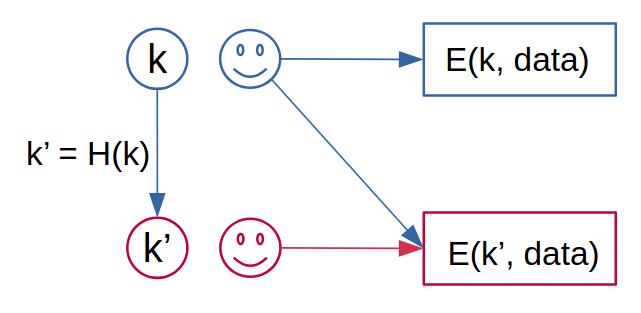
\includegraphics[width=0.45\textwidth]{img/one_way.png}
    \end{figure}
    
    Dato in input una chiave, ottengo in output un'altra chiave $k' = H(k)$ in questo caso cosa dovrebbe rompere Eve per riuscire a decifrare? In questo contesto anche se $H$ \textbf{non} è \textit{collision resistance} non è di interesse infatti anche se si trovasse un $k'' \; \text{t.c.} \; k' = H(k'') \rightarrow k \neq k''$ e quindi Eve non riuscirebbe a rompere lo schema crittografico di cifratura, l'unico modo per Eve di ottenere il dato in chiaro è riuscire a trovare una funzione $H^{-1} \; \text{t.c.} \; k = H^{-1}(k')$ e utilizzarla per decifrare le informazioni di Alice - ci basta: \textbf{\textit{One Way}}. \\
    L'unica limitazione è che se l'input $k$ è debole e quindi vulnerabile a \textit{brute-force} allora sarebbe possibile eseguire una ricerca esaustiva nell'insieme delle chiavi - \textbf{\textit{HKDF}}.

    \medskip

    \textcolor{red}{\textbf{\textit{Second pre-Image Collision Resistance}}}: dato un $d$ e un $m$ tale che $d = H(m)$ trovare un valore $m' \; \text{t.c.} \; d = H(m')$ è tecnicamente richiesta per gli \textbf{\textit{authentication schemes}} ad esempio nel contesto di \textbf{\textit{Keyed Hash Function}} - per l'offuscamento di password su DB - infatti riuscendo o a trovare $H^{-1}$ o trovando un'altro valore $m'$ che generi lo stesso \textit{digest} è possibile bypassare il controllo.
\end{flushleft}

\begin{boxA}
    \textcolor{orange}{\textbf{Esempio}}: \textbf{Download di dati}

    \medskip

    {\centering
        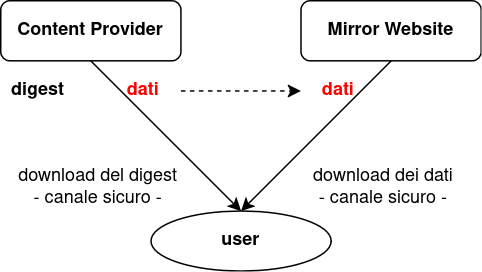
\includegraphics[width=0.45\textwidth]{img/hash_es.png}
    \par}

    Quando un sito mette a disposizione dei dati per il download - ad esempio un \textit{*.iso}, normalmente il contenuto per il download è disponibile su un \textit{server mirror}, quindi il \textit{provider} si calcola il \textit{digest} $d = H(m)$ e poi fa l'upload del contenuto sul \textit{server mirror}. L'utente si scarica il contenuto dal \textit{server mirror} e scarica il \textit{digest} dal \textit{provider}, successivamente calcola l'hash del dato scaricato $d_u = H(m_d)$ se e solo se $d_u = d$ accetta il dato scaricato.

    \smallskip

    In questo caso la funzione hash $H$ deve rispettare la ``normativa'' di sicurezza \textit{second pre-image collision resistance} in quanto il messaggio iniziale - la nostra \textit{*.iso} - viene fornita dal \textit{server mirror}. L'attaccante vincerebbe se riuscisse a trovare un messaggio $m_a \; \text{t.c.} \; H(m_d) = H(m_a)$ e contemporaneamente quel messaggio dovrebbe contenere un \textit{payload} malevolo. Solo in quel caso l'utente lo scaricherebbe il messaggio e la funzione di verifica - chiamata \textbf{\textit{verify}} - andrebbe a buon fine e quindi l'utente accetterebbe il nuovo messaggio.
\end{boxA}

\begin{flushleft}
    \textcolor{red}{\textbf{\textit{Collision Resistance}}}: riuscire ad ottenere, arbitrariamente, due messaggi $m_1$ e $m_2$ tali che $H(m_1) = H(m_2)$ è la più forte come garanzia di sicurezza, nel caso dovesse mancare, la funzione hash sarebbe molto facile da violare.
\end{flushleft}

\begin{boxA}
    \textcolor{orange}{\textbf{Esempio}}

    \medskip

    {\centering
        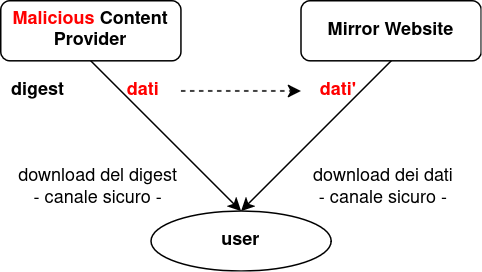
\includegraphics[width=0.45\textwidth]{img/hash_es_2.png}
    \par}

    Il \textit{provider} è malevolo e riesce a trovare due messaggio $m$ e $m'$ tali che $H(m) = H(m')$ a questo punto fa l'upload del messaggio malevolo sul \textit{server mirror}, l'utente che si scarica riesce a verificare la correttezza del \textit{digest}.
\end{boxA}

\begin{flushleft}
    \textcolor{red}{\textbf{\textit{Hash Function Security Parameters}}}: il \textbf{parametro di sicurezza} delle funzioni \textit{hash} è la \textbf{lunghezza del \textit{digest}} in quanto rappresenta le prossibili combinazioni di $n$ bit, ovvero i possibili valori prodotti dalla funzione \textit{hash} ($2^n$). Come discusso nel paragrafo di sicurezza computazionale, il valore di $n$ deve essere scelto considerando l'attacco noto più efficiente, analizzando anche il numero di operazioni richieste per trovare una collisione. 

    \smallskip

    Una funzione hash sicura è quello in cui l'attacco più efficiente per trovare una collisione è il \textbf{\textit{Birthday Attack}} che richiede $2^{n/2}$ ovvero la probabilità di trovare una collisione è del $50\%$ su $N$ ($\sqrt{N}$)

    \medskip

    Alcune delle più popolari funzioni hash:
    \begin{itemize}[nosep]
        \item \textbf{md5}: ad oggi deprecata, molto facile trovare delle collisioni.
        \item \textbf{sha1}: anche questa ad oggi deprecata, vi sono trovate delle collisioni. 160bit di \textit{digest}.
        \item \textbf{sha2}: sha1 ``potenziata'' ha diverse lunghezze del \textit{digest} in base alla versione: \textbf{sha224}, \textbf{sha256}, \textbf{sha384} e \textbf{sha512}.
        \item \textbf{sha3}: è stata implementata con una primitiva differente rispetto a sha1 e sha2, è stata standardizzata ufficialmente nel 2015, ha le stesse sottoversioni del sha2.
        \item \textbf{blake2}: utilizza come primitiva \textbf{chacha} non è ancora stata standardizzata dal NIST ma è molto popolari in certi ambienti, ad esempio, quello del \textit{software open source}.
    \end{itemize}

    Sia le funzioni \textbf{\textit{hash}} che le funzioni \textbf{\textit{mac}} vengono definite come funzioni con un solo input, ma è possibile concatenare più input, ma bisogna farlo in maniera sicura.

    {\centering
        $H('builtin' || 'security') = H('built' || 'insecurity') = H('builtinsecurity')$
    \par}

    Concatenare i risultati cercando di rendere univoco l'output:
    \begin{itemize}[nosep]
        \item utilizzando \textbf{caratteri speciali} per concatenare, se possibile: considersiamo che il carattere $;$ non sia ammesso come input allora sarà possibile concatenare gli input come: $d = H('builtin' \; || \; ';' \; || \; 'security')$
        \item \textbf{esplicitando} la \textbf{lunghezza dell'input}: $d = H('7buildinsecurity')$ 
    \end{itemize}
\end{flushleft}

\section{Message Authentication Code}

\begin{flushleft}
    Il destinatario può rilevare se il messaggio non è stato mandato da un mittente legittimo, che nel caso lo si andasse a definire all'interno della crittografia simmetrica, identificherebbe colui che conosce il segreto condiviso. Il \textbf{MAC} è una funzione che ha due input: la chiave e il message e come output un \textbf{\textit{tag}}.

    {\centering
        \textbf{tag} = \textbf{MAC}(\textit{key}, \textit{message})
    \par}

    La funzione \textbf{\textit{verify}} è simile a quella delle funzioni hash, ma include come input anche la chiave simmetrica.

    {\centering
        $\{0, 1\} \leftarrow$ \textbf{verify}(\textit{key}, \textit{message}, \textit{tag})
    \par}

    Il \textbf{MAC} permette a Bob di verificare che il messaggio è stato generato da Alice.
\end{flushleft}

\begin{flushleft}
    \textcolor{red}{\textbf{\textit{Attack Models for MAC}}}

    \medskip

    \begin{minipage}[c]{0.45\textwidth}
        \centering
        \textbf{\textit{Existential Forgery for Passive Eavesdropper}} \\
        L'attaccante osserva coppie $(m_i, t_i)$ trasmesse tra gli attori benevoli (Alice e Bob) ed è capace di \textit{forgiare} una nuova coppia $(m', t')$ mai inviata e l'attacco ha successo nel caso in cui il messaggio venga accettato.

        \smallskip

        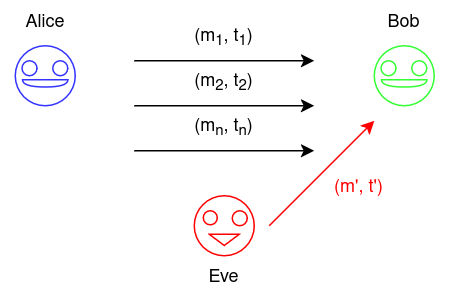
\includegraphics[width=\textwidth]{img/mac_am_1.png}
    \end{minipage}
    \hfill
    \begin{minipage}[c]{0.45\textwidth}
        \centering
        \textbf{\textit{Existential Forgery for Chosen Message}} \\
        In questo caso l'attaccante controlla i messaggi che vengono autenticati, quindi sceglie $n$ volte un messaggio $m_i$ e osserva il tag generato $t_i$ a quel punto se riesce a generare una nuova coppia $(m', t')$ non ancora inviata che verrà accettata l'attacco avrà avuto successo.

        \smallskip

        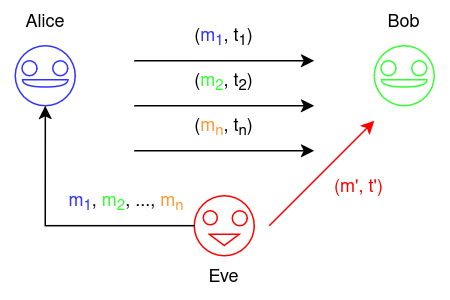
\includegraphics[width=\textwidth]{img/mac_am_2.png}
    \end{minipage}

    \smallskip

    \textcolor{red}{\textbf{\textit{MAC: Security Parameters}}}:
    \begin{itemize}[nosep]
        \item la \textbf{lunghezza della chiave}: l'attacco più efficiente deve essere quello di \textit{brute force}.
        \item la \textbf{lunghezza del \textit{tag}}: permette di determinare la dimensione del dato o il numero di messaggi autenticabili con la stessa chiave (dipende dal tipo di \textbf{\textit{MAC scheme}} che si vuole utilizzare). Ricordiamo che il \textit{tag} è \textbf{\textit{overhead}} sul messaggio e quindi è possibile minimizzarlo ma aggiungendo a livello di protocollo altri fattori di sicurezza. 
    \end{itemize}

    La scelta del \textbf{MAC} dipende dai requisiti nei quali va applicato. Disponibilità software (presenza di librerie), disponibilità hardware (accelleratore hardware) e l'abilità di soddisfare requisiti degli schemi (creare \textit{nonce}). Ogni tipologia di \textbf{MAC} offre un diverso \textit{trade-offs} in termini di: lunghezza e numero di messaggi, modelli di attacco e lunghezza del tag consentita.

    \medskip

    Consideriamo i \textbf{MAC} all'interno di una situazione di \textcolor{red}{\textbf{\textit{Replay Attack}}}. Abbiamo detto che il \textbf{MAC} può garantire che il \textit{tag} sia stato creato con una certa \textbf{chiave simmetrica}, ma nel contesto in cui siamo Eve re-invia lo stesso messaggio che ha inviato Alice a Bob, che è valido, perché creato da Alice - se Alice e Bob fossero due banchieri e Alice inviasse un messaggio con scritto "Aggiungi 1000 euro nell'account di Carlo". Con queste tipologie di attacco utilizzando la crittografia è difficile arginarle, è possibile però metterci una ``pezza'' lato architetturale (a livello \textbf{trasporto} o \textbf{applicazione}) ad esempio aggiungendo un \textbf{contatore univoco} al messaggio:
    
    {\centering
        \textbf{m} = (id=n, data), tag
    \par}

    Se consideriamo che la comunicazione sia \textit{full-duplex} - \textbf{\textit{Reflection Attacks}} - la possibilità che il messaggio venga inviato al mittente dello stessa e che venga verificato il \textit{tag} non è nulla, quindi si è aggiunto un bit di direzione del messaggio:

    {\centering
        \textbf{m} = (id=n, dir=val, data), tag
    \par}

    Il bit di direzione è aggiunto come \textbf{metadato} per un verifica ulteriore da parte del destinatario. È anche possibile utilizzare una difesa diversa, gestire la comunicazione \textit{full-duplex} come due \textbf{comunicazioni sicure \textit{half-duplex}} quindi utilizzare due \textbf{chiavi differenti} entrambe condivise, ma se invia Alice, verrà utilizzata $k_1$, se invia Bob $k_2$.

    \medskip

    \textcolor{red}{\textbf{\textit{MAC \& Hash function}}} \\
    Consideriamo un \textit{tag} generato in questo modo: \textbf{H}(\textbf{key} || \textbf{message}), ovvero ci calcoliamo l'hash di una stringa generata concatenando la chiave con il messaggio. Si potrebbe pensare che se la funzione hash è \textit{collision resistance} un'attaccante non riuscirebbe a calcolare un \textit{digest} la cui pre-immagine è (parzialmente) sconosciuta. In verità questo tipo di costrutto è vulnerabile al \textbf{\textit{length extension attack}} in quanto molte funzioni hash si basano sulla primitiva di \textbf{\textit{Merkle-Damgard}} (non vale per \textbf{sha3})
\end{flushleft}

\begin{boxA}
    \textcolor{red}{\textbf{\textit{Merkle-Damgard Design}}} \\

    {\centering
        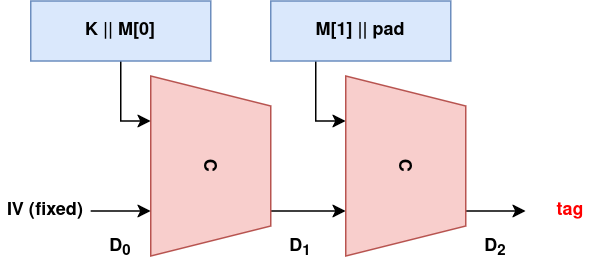
\includegraphics[width=0.45\textwidth]{img/hash_md.png}
    \par}

    È la primitiva che viene utilizzata da \textit{hash function} come \textbf{md5}, \textbf{sha1}, \textbf{sha2}. Considerando la figura, vediamo che:
    \begin{itemize}[nosep]
        \item \textbf{K} è il segreto.
        \item \textbf{M[0]} e \textbf{M[1]} è pubblico.
        \item la costruzione del \textbf{pad} è pubblica.
        \item $D_2$ è pubblico (\textbf{\textit{tag}})
    \end{itemize}
    In questa circostanza l'attaccante vince se riesce a generare un \textit{tag} valido per un certo messaggio arbitrario senza conoscere la chiave \textbf{K}. Noi (come attaccante) sappiamo che il \textit{tag} è generato \textbf{H}(\textbf{key} || \textbf{message}) dove \textbf{K} è un segreto con una data lunghezza \textbf{l} fissata, noi vogliamo calcolare un certo \textit{tag'} che venga generato \textbf{H}(\textbf{key} || \textbf{message} || \textbf{message'}).
    \begin{enumerate}[nosep]
        \item Consideriamo di utilizzare la stessa \textit{hash function}, e di ripristinare il suo stato interno come, quindi ponendo come nostro \textbf{IV} il \textit{tag} generato dalla computazione legittima, ma è necessario impostare anche il punto iniziale da dove andare a calcolare il \textbf{pad'} e deve essere pari a $len(K) + len(M) + len(pad)$.
        \item Inviamo come messaggio \textbf{M || pad || M'} e come tag quello appena calcolato \textbf{\textit{tag'}}.
        \item il destinatario calcolerà \textbf{H}(\textbf{K} || \textbf{pad} || \textbf{M} || \textbf{pad} || \textbf{M'}) e produrrà lo stesso \textit{tag'} 
    \end{enumerate}
\end{boxA}

\begin{flushleft}
    \textcolor{red}{\textbf{\textit{HMAC}}}: è un MAC che viene costruito con alla base una funzione hash (alcune volte chiamato \textbf{\textit{keyed-hash function}}), è necessario che mantenga due requisiti funzionali:
    \begin{itemize}[nosep]
        \item il \textbf{MAC} deve essere sicuro fintanto che la primitiva hash su cui è costruito è \textit{collision resistance}.
        \item per molti degli scenari presi in considerazione è sufficiente una \textit{second pre-image collision resistance}
    \end{itemize}
    Viene definito come:

    {\centering
        \textbf{HMAC}(\textbf{K}, \textbf{M}) = \textcolor{blue}{\textbf{H(}}(Kp $\oplus$ opad) || \textcolor{red}{\textbf{H(}}(Kp $\oplus$ ipad) || (m)\textcolor{red}{\textbf{)}}\textcolor{blue}{\textbf{)}}
    \par}
    Dove: 
    \begin{itemize}[nosep]
        \item \textbf{K} è un segreto a lunghezza variabile, mentre \textbf{Kp} è la sua versione \textit{zero-padded}.
        \item \textbf{opad}(\textbf{\textit{outer padding}}) e \textbf{ipad}(\textbf{\textit{inner padding}}) sono costanti con un elevata distanza di Hamming (ovvero che le posizioni di bit diversi sono elevate), utilizzate per consentire alle due funzioni hash di utilizzare chiavi diverse.
    \end{itemize}
\end{flushleft}

\begin{flushleft}
    Andiamo a considerare i \textbf{MAC} costruiti su \textit{block cipher}, il primo e il più semplice per costruire un \textbf{MAC} basato su \textit{block cipher} fu quello di utilizzare la \textbf{CBC} \textit{mode of operation} e utilizzare come \textit{tag} il testo cifrato dell'ultimo blocco.

    {\centering
        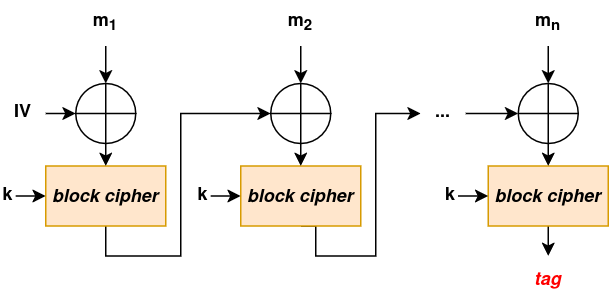
\includegraphics[width=0.45\textwidth]{img/cbc_mac.png}
    \par}

    È possibile \textit{forgiare} un messaggio, da parte di un attaccante, infatti dato \textbf{(m, t)} e \textbf{(m', t')}, un \textcolor{red}{\textbf{CBC-MAC}} producerà \textbf{t'} per un messaggio costruito come: \textbf{m || t $\oplus$ m' || m'}.

    \medskip
    
    \textcolor{red}{\textbf{\textit{CMAC}}} è il successore del \textbf{CBC-MAC} utilizza come primitiva \textbf{AES-SIV}(\textbf{CTR-CMAC}), lo schema è molto simile ma aggiunge due operazioni sull'ultimo blocco prima di utilizzarlo. Lo schema deriva due chiavi $k_1$ e $k_2$ dalla chiave originale e una delle due viene \textit{xorata} con l'ultimo blocco del messaggio $m_n$ (\textbf{\textit{tweak block}}) prima di utilizzare il blocco del \textbf{CMAC}.

    {\centering
        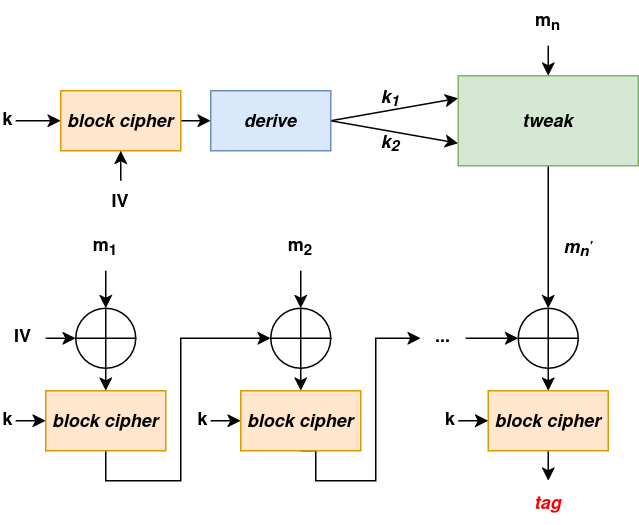
\includegraphics[width=0.45\textwidth]{img/cmac.png}
    \par}

    \newpage

    \textcolor{red}{\textbf{\textit{UHF - Universal Hash Function}}} si riferisce ad una \textbf{\textit{keyed hash function}} che prende due input: una chiave \textbf{k} e un messaggio \textbf{m}. Questa funzione garantisce che la probabilità - che dati due messaggi distinti $m_1$ e $m_2$ - di avere $UHF(m_1) = UHF(m_2)$ è \textbf{trascurabile}. Un'implementazione popolare per una funzione \textbf{UHF} è quella basata su \textbf{polinomi modulo p} (con \textbf{p} primo):
    \begin{itemize}[nosep]
        \item scegliamo un primo \textbf{p}
        \item consideriamo il messaggio $m$ come un vettore di interi in $\mathbb{Z}_p$ con un massimo di $n$ elementi: $m = [m_1, m_2, ..., m_n]$
        \item la funzione hash \textbf{H} viene calcolata utilizzando gli elementi di $m$ come coefficienti del polinomio $F(k)$:
        
        {\centering
            $H(k, M) = \overset{n}{\underset{i=1}{\sum}} (m_i \cdot k^i) \mod p$
        \par}

    \end{itemize}

    \medskip
    
    \textcolor{red}{\textbf{\textit{One-Message Polynomial evaluation MACs}}}: è possibile costruire un \textbf{MAC} partendo da delle \textbf{UHF}, consideriamo il messaggio $m = m_1, m_2, ..., m_n$

    {\centering
        $mac(m, k, r) = r + H(m, k) = r + \overset{n}{\underset{i=1}{\sum}} (m_i \cdot k^i) \mod p$
    \par}

    In questo caso il \textbf{MAC} è un polinomio di grado $n$, \textbf{p} è fissato ed è pubblico, se $m_i$ è 128bit allora $p > 128$. \textbf{k} e \textbf{r} vengono scelti randomicamente:
    \begin{itemize}[nosep]
        \item \textbf{k} lavora come la chiave per la computazione, può essere utilizzata per più messaggi.
        \item \textbf{r} ha la stessa funzionalità di un \textbf{\textit{nonce}} random, e bisogna utilizzarlo assolutamente per un unico messaggio, in questo caso \textbf{r} è \textbf{segreto}.
    \end{itemize}
    Nel caso in cui \textbf{r} venisse ripetuto per due \textit{tag}:
    \begin{align*}
        \mathbf{t_1} &= mac(m_1, k, r) = r + H(m_1, k) \\
        t_1 - r - H(m_1, k) &= 0 \\
        \mathbf{t_2} &= mac(m_2, k, r) = r + H(m_2, k) \\
        t_2 - r - H(m_2, k) &= 0
    \end{align*}

    \begin{align*}
        t_1 - \cancel{r} - H(m_1, k) &= t_2 - \cancel{r} - H(m_2, k) \\
        \overset{n}{\underset{i=1}{\sum}}(m_{1,i} \cdot k^i) + t_1 &= t_2 + \overset{n}{\underset{i=1}{\sum}}(m_{2,i} \cdot k^i) \\
        \overset{n}{\underset{i=1}{\sum}}((m_{1, i} - m_{2, i}) \cdot k^i) + t_1 - t_2 &= 0 \mod p
    \end{align*}
    In questo modo la chiave \textbf{k} è tra le radici del polinomio $m_2 - m_1 + t_1 + t_2$. 
    \smallskip
    È possibile estendere \textit{one-message poly MACs} ad un \textit{multi-message} utilizzando o una \textbf{PRF} oppure \textbf{PRP} (ad esempio un \textit{block cipher}), in questo modo, invece che utilizzare un valore di \textbf{r} random possiamo calcolarlo partendo da una chiave e un \textit{nonce}:

    {\centering
        $mac(m, k = \langle k_1, k_2 \rangle, n) = AES(n, k_1) + H(m, k_2)$
    \par}

    Se $k_1$ è segreta, un avversario, non sarebbe in grado di calcolarsi \textbf{AES}(n, $k_1$) anche se il valore $n$ fosse pubblico e non randomico, ma utilizzare lo stesso \textit{nonce} più volte esporrebbe $k_2$ e quindi romperebbe lo schema.

    \medskip

    \textcolor{red}{\textbf{\textit{GMAC}}} è basato su \textbf{AES-GCM} e in questo caso i rischi per la sicurezza in caso di errori di utilizzo sono molto più elevati a causa del comportamento lineare della funzione. Richiede un \textbf{\textit{unpredictable nonce}}, riutilizzare lo stesso \textit{nonce} per firmare messaggi diversi permette la \textbf{\textit{key recovery}}, in questo caso è molto importante utilizzare la variante \textbf{SIV} - molto più robusti a discapito delle \textit{performance} - come primivita dello schema (\textbf{AES-GCM-SIV}). La probabilità di successo in caso di attacco \textbf{aumenta} all'\textbf{aumentare della dimensione del messaggio}.

    \smallskip

    Non possiamo effettuare un'analisi a \textit{black-box} per definire come la dimensione del \textit{tag} influenzi il \textbf{livello di sicurezza}. Il dimensionamento richiede la conoscenza dello schema e le analisi sono parecchio complesse. Alcuni esempi:
    \begin{itemize}[nosep]
        \item \textbf{HMAC} e \textbf{CMAC}: è possibile mandare un numero di messaggi pari alla radice quadrata della dimensione del \textit{digest}
        \item \textbf{GHASH} (e \textbf{GMAC}): il numero dei messaggi è lineare con la dimensione del \textit{digest}, ma diminuisce rispetto alla dimensione di ogni messaggio.
        \item \textbf{Poly1305}: rappresenta un \textit{trade-off}, alto numero di messaggi dimensionalmente limitati.
    \end{itemize}
\end{flushleft}
\chapter{Security Guarantees \& Attack Model \\ \small{for Symmetric Encryption}}

\begin{flushleft}
    Ogni schema crittografico garantisce sicurezza contro un certo attaccante a condizione che siano soddisfatti certi requisiti:
    \begin{itemize}[nosep]
        \item dobbiamo decidere quale modello si adatta allo schema considerato.
        \item dobbiamo considerare i vincoli funzionali e non.
    \end{itemize}

    Lo scopo finale dell'attaccante è quello di violare la \textbf{confidenzialità}, per ora abbiamo solo considerato un attaccante che non ha alcuna conoscenza \textbf{EAV}, ma a volte, l'attaccante può anche:
    \begin{itemize}[nosep]
        \item avere \textbf{conoscenza} aggiuntiva sul \textit{plaintext}.
        \item violare l'\textbf{integrità} di un vettore di attacco per ottenere delle informazioni.
        \item \textbf{interagire} con le parti fidate.
    \end{itemize}

    È importante ricordare che la confidenzialità nella crittografia moderna è modellata come \textbf{indistinguibilità} da una sequenza random. Infatti l'avversario vince nel caso in cui è capace di riconoscere un crittogramma da un messaggio random con una proabilità maggiore del $50\% + negl(n)$

    \smallskip

    Non è possibile enumerare tutti i possibili attacchi di uno scenario reale, quello che si prefigge la crittografia moderna è considerare alcuni modelli formali contro i quali la sicurezza degli schemi crittografici è comprovata. Il che ci permette di progettare il protocollo o l'applicazione andando a scegliere il modello più adatto al proprio scenario. Gli schemi di sicurezza sono dimostrati sicuri in presenza di determinati modelli di attacco.

    \medskip

    \textcolor{red}{\textbf{\textit{Attack Model}}} \\
    I modelli di attacco vegono pensati basandosi su due criteri di misura: \textbf{\textit{knowledge}} - che cosa sa l'avversario del nostro sistema - \textbf{\textit{attack surface}} - quali interfacce espone il nostro sistema che anche un avversario potrebbe utilizzare.

    \smallskip

    La crittografia formale moderna chiama queste interfacce \textbf{oracoli}, e normalmente andiamo a definirne di due tipologie:
    \begin{itemize}[nosep]
        \item \textbf{\textit{encryption oracle}}: l'attaccante può dare \textbf{input} all'oracolo e gli verrà ritornato un dato cifrato in \textbf{output} che corrisponde a \textbf{E}(input).
        \item \textbf{\textit{decryption oracle}}: è il duale dell'\textit{encryption oracle}.
    \end{itemize}
    Un vincolo aggiuntivo che si può aggiungere alla superficie di attacco quando si considera la distribuzione di un applicativo nel mondo reale è la tipologia di computazione che deve eseguire un attaccante: \textbf{\textit{online}} - l'interazione è con l'oracolo - e \textbf{\textit{offline}} - non è necessario consultare l'oracolo.

    \smallskip

    \textcolor{red}{\textbf{\textit{Attack Models} Differenti}}
    \begin{center}
        \begin{minipage}[c]{0.75\textwidth}
            \begin{itemize}[nosep]
                \item \textbf{\textit{Eavesdropper - EAV}} anche nota come \textbf{\textit{Ciphertext-Only Attack - COA}} l'avversario è passivo e non ha conoscenza sui crittogrammi che riesce ad intercettare.
                \item \textbf{\textit{Known-Plaintext Attack - KPA}} in questo caso l'avversario ha la conoscenza della coppia $(p_i, c_i)$
                \item \textbf{\textit{Chosen-Plaintext Attack - CPA}} 
                l'attaccante ha accesso ad una \textit{encryption interface} e quindi è in grado di cifrari messaggi arbitrari.
                \item \textbf{\textit{Non-Adaptive Chosen-Ciphertext Attack - CCA1}}: l'avversario ha accesso ad una \textit{decryption interface}, ma accesso limitato al risultato e limite sul numero di \textit{query} che può eseguire.
                \item \textbf{\textit{Adaptive Chosen-Ciphertext Attack - CCA2}}: l'avversario ha accesso ad una \textit{decryption interface} e anche al risultato e quindi modificare l'attacco in base ai risultati.
            \end{itemize}
        \end{minipage}
        \hfill
        \begin{minipage}[c]{0.1\textwidth}
            \centering
            \begin{tikzpicture}[scale=1]
                \node[rotate=270, anchor=south, text=red] at (0,2.2) {\textbf{stronger attack models}};
                \draw[<-, thick, black] (0,-3.0) -- (0,7.0);
            \end{tikzpicture}
        \end{minipage}
    \end{center}

    Come detto in precedenza la \textbf{confidenzialità} in crittografia modeerna equivale a dire che il crittogramma prodotto è \textbf{indistinguibile} da un \textit{random bitstring}. Associando \textbf{IND} ad un modello di attacco andiamo a definire una \textbf{garanzia di sicurezza} dello schema preso in considerazione, ad esempio dire che il nostro schema di crittografia è \textbf{IND-CPA} significa che lo schema è \textbf{indistinguibile da un \textit{random} contro un modello di attacco \textit{Chosen-Plaintext Attack}}.

    \smallskip

    \textcolor{red}{\textbf{IND-EAV (\textit{Indistinguishably under Eavesdropper Attack})}}: è la tipologia di attacco più debole, in quanto un attaccante non sa nulla. Eve è un attaccante passivo che osserva crittogrammi senza eseguire alcuna modifica su di essi e senza interagire con le parti fidate, ma soprattutto senza alcuna conoscenza del testo in chiaro.
\end{flushleft}

\begin{boxA}
    \textcolor{red}{\textbf{\textit{Semantic Security Games on IND-COA}}} \\
    Tutti i \textit{security games} per la confidenzialità sono basati sul concetto di \textbf{indistinguibilità}, un algoritmo eseguito dall'attaccante che ha come scopo di distinguere informazioni dal \textit{plaintext}. 
    
    \smallskip

    Nel modello di attacco \textbf{COA}, l'avversario legge i crittogrammi in transito e prova a indovinare il bit successivo. Riuscirà a vincere il gioco solo se ha un \textit{distinguisher} che indovina il bit corretto con una probabilità $ > 0.5$, nei moderni modelli di attacco, l'avversario non deve necessariamente ottenere la chiave di cifrazione o il contenuto effettivo del testo in chiaro affinché uno schema si consideri ``rotto''.
\end{boxA}

\begin{flushleft}
    \textcolor{red}{\textbf{IND-KPA (\textit{Indistinguishably under Know-Plaintext Attack})}}: Eve è un attaccante passivo che osserva i crittogrammi senza eseguire alcuna modifica su di essi e senza interagire con le parti fidate, ma può conoscere vecchie corrispondenze tra $m$ e $c$ o informazioni sullo spazio dei testi in chiaro, come la distribuzione statistica.
    
    \smallskip

    \textcolor{red}{\textbf{IND-CPA (\textit{Indistinguishably under Chose-Plaintext Attack})}}: è la sicurezza minima richiesta da tutti i moderni crittosistemi, l'attaccante viene modellato per avere accesso ad un \textit{encryption oracle}.

    {\centering
        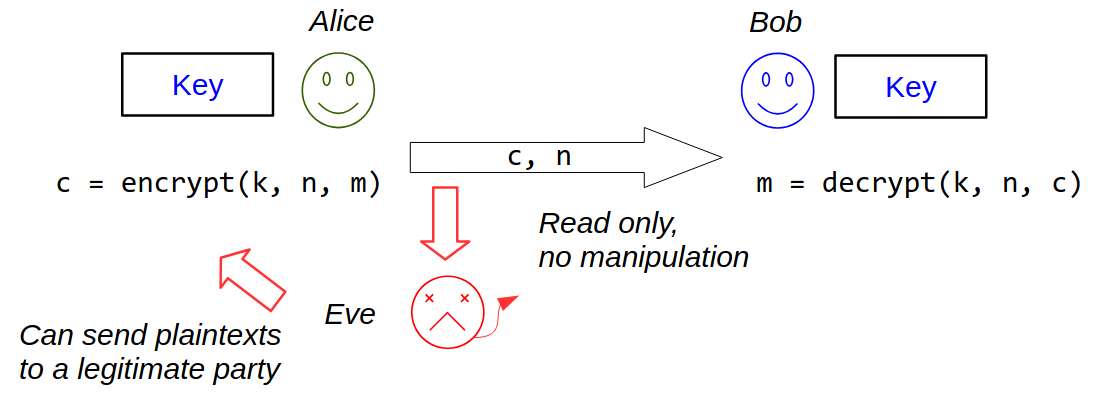
\includegraphics[width=0.45\textwidth]{img/ind_cpa.png}
    \par}

    \textbf{\textit{Security Games}}
    \begin{enumerate}[nosep]
        \item il \textbf{\textit{challenger}} genera una chiave segreta.
        \item l'\textbf{\textit{adversary}} sceglie due messaggi $m_0$ e $m_1$ della stessa lunghezza e gli invia al \textit{challenger}.
        \item il \textit{challenger} genera randomicamente un bit $b \leftarrow \{0, 1\}$ e genera $c = E(m_b)$ e lo invia all'avversario.
        \item l'\textit{adversary} analizza il crittogramma e può scegliere se ripetere gli step dal secondo o passare al quinto.
        \item l'avversario espone come output un valore $b \leftarrow \{0, 1\}$ in base a quale messaggio - se $m_0$ o $m_1$ - è il corrispondente di $c$.
    \end{enumerate}
    L'\textit{adversary} vince il gioco se è capace di riconoscere con una probabilità $ > 0.5\% + negl(l)$ a quale messaggio corrisponde il crittogramma ricevuto.
    
    \smallskip

    Qualunque schema \textbf{deterministico} è intrinsecamente vulnerabile a un attacco del tipo \textbf{IND-CPA}, in quanto basterebbe all'attaccante ripetere lo stesso messaggio per un più iterazioni consecutive e vincere, infatti schemi crittografici sono sicuri sotto la modellazione \textbf{\textit{Distinc Chosen-Plaintext Attack - DCPA}} che obbligano l'\textit{adversary} a scegliere una coppia di messaggi diversi per ogni iterazione del \textit{security game}. Crittografia deterministica è spesso implementata fornendo \textit{nonce} o \textit{IV} fissi (costanti) allo schema, cercando di evitare schemi che sono vulnerabili contro \textit{re-use} di \textit{nonce} o \textit{IV} oppure preferendo schemi che utilizzano \textbf{SIV}. \\
    \textbf{\textit{Deterministic Encryption with Associated Data - DAEAD}} framwork.
\end{flushleft}

\begin{boxA}
    \textcolor{red}{\textbf{IND-CPA e il requisito di impredicibilità dell'IV in CBC}}
    \begin{itemize}[nosep]
        \item \textit{adversary}: sceglie un $m$ che ha lunghezza pari alla \textit{block size} del \textit{block cipher} e lo invia.
        \item \textit{challenger}: sceglie un \textit{IV} e calcola il \textit{ciphertext} $c$, ritornando la coppia $(c, iv)$.
    \end{itemize}
    Facciamo ora un'\textbf{assunzione}: l'avversario conosce l'\textit{IV} successivo - \textbf{\textit{predictable IV}}. \\
    L'avversario può calcolarsi un messaggio $m'$ come $m' = (m \oplus iv \oplus iv')$ dove \textbf{\textit{iv'}} è l'\textit{IV} successivo che utilizzerà il \textit{challenger}. Se il \textit{challenger} cifrerà il messaggio 
    
    {\centering
        $c' = E(iv', m') = E(m' \oplus iv', k) = E(m \oplus \cancel{iv'} \oplus iv \oplus \cancel{iv'}, k) = E(m \oplus iv, k) = c$
    \par}
\end{boxA}

\begin{flushleft}
    \textcolor{red}{\textbf{\textit{IND-CCA1 (Indistinguishably under Chosen-Ciphertext Attack)}}} permette di difendersi contro attacchi attivi sul crittogramma. L'attaccante è capace di manipolare il \textit{ciphertext} al \textit{decryption oracle} (gli input dell'attaccante non sono adattivi per via della definizione data).

    {\centering
        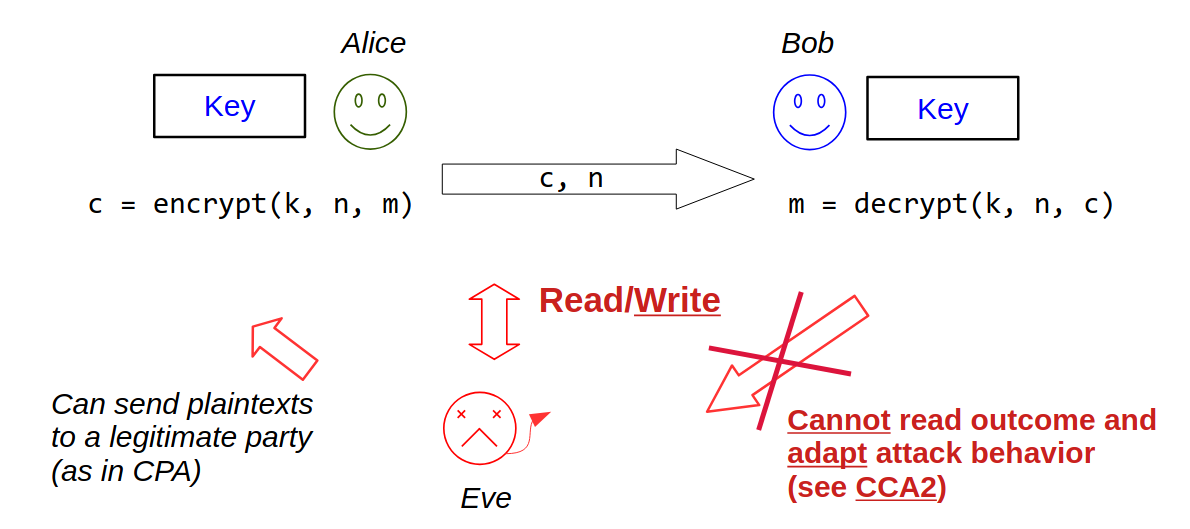
\includegraphics[width=0.45\textwidth]{img/ind_cca1.png}
    \par}

    \textbf{IND-CCA} coinvolge anche \textbf{modifiche al crittogramma} e \textbf{attacchi all'integrità per violare la confidenzialità}. 

    \smallskip

    \textcolor{red}{\textbf{\textit{Malleability}}} si riferisce alla capacità di un'attaccante di ricotruire quali bit del crittogramma sono influenzati dalla modifica di un bit nel testo in chiaro.

    \smallskip

    Un schema crittografico basato su \textcolor{red}{\textbf{\textit{stream cipher}}} viene definito \textbf{\textit{fully malleable}} in quanto una modifica nel testo cifrato in una certa posizione $c_i$ porta ad una modifica nel testo in chiaro nella medesima posizione $p_i$, ad esempio:
    \begin{enumerate}[nosep]
        \item \textit{flipping} il \textbf{bit di direzione} in uno protocollo di comunicazione per eseguire un \textbf{\textit{reflection attack}}.
        \item \textit{flipping} il numero di versione per effettuare un \textbf{\textit{downgrade attack}}.
    \end{enumerate}

    \smallskip

    Per ottenere una certa garanzia di \textbf{integrità} (senza utilizzare \textbf{MAC}) è necessario ricorrere a modalità di crittografia basate su \textit{block cipher}. Andiamo ad osservare il comportamento di uno schema crittografico basato su un qualunque \textit{block cipher} ma che abbia come \textit{mode of operation} \textbf{CBC}, in questo caso analizzando lo schema per decifrare un crittogramma generato, ad esempio, con \textbf{AES-CBC} è fattibile modificare l'\textit{IV}.

    {\centering
        
\includegraphics[width=0.45\textwidth]{img/ind_cca1_cbc.png}
    \par}

    Assumiamo che l'attaccante conosca il testo originale $p$ e voglia che in decifrazione venga generato il testo $p'$, nel \textbf{primo blocco}, allora sarebbe possibile calcolarsi un \textit{IV} tale che $IV' = (IV \oplus p \oplus p')$ e sostituire l'\textit{IV} originale con quello generato, in quel caso il primo blocco sarebbe $p'$ e i restanti blocchi rimerrebbero invariati.

    \medskip

    \textcolor{red}{\textbf{\textit{IND-CCA2 (Indistinguishably under Adaptive Chosen-Ciphertext Attack)}}} difende da attacchi attivi iterati e potenzialmente illimitati (l'attaccante è ancora \textbf{polinomiale}), in cui l'attaccante adatta i suoi attacchi in base alla risposta di Bob. L'attaccante invia un testo cifrato manipolato al \textit{decryption oracle}.

    {\centering
        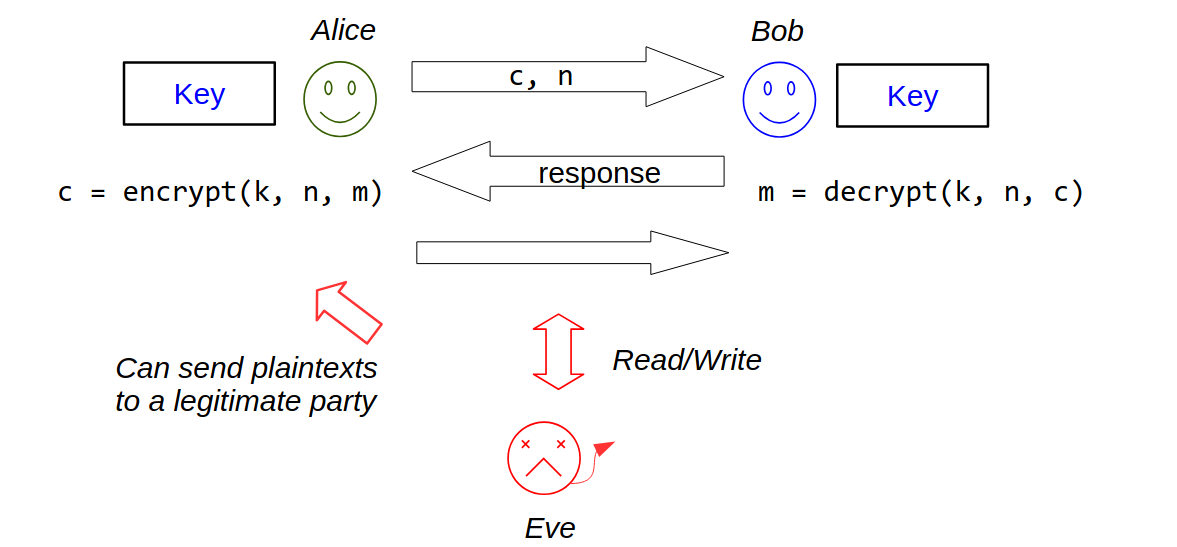
\includegraphics[width=0.45\textwidth]{img/ind_cca2.png}
    \par}
\end{flushleft}

\begin{boxA}
    \textcolor{red}{\textbf{\textit{Padding Oracle Attack}}} \\
    Consideriamo un attacco alle funzioni di \textbf{decifrazione} e \textbf{\textit{unpadding}}, l'attacco ha successo se riusciamo a generare un crittogramma che decifrandolo ha la struttura del \textit{padding} corretto. Gli attacchi al \textit{padding} mirano a manipolare un blocco di un crittogramma $c[i]$ per manipolare il blocco successivo di \textit{plaintext} $p[i+1]$. È simile alla manipolazione dell'\textit{IV} ma in questo caso andiamo a considerare gli ultimi due blocchi del \textit{ciphertext}, modificare il penultimo blocco per manipolare l'ultimo. In questo caso non abbiamo la certezza di come manipolare il crittogramma, ma possiamo \textit{guessare} - questo comporta che, in caso, di un unico tentativo ci siano probabilità trascurabili di successo, se avessimo più tentativi rientraimo nei \textbf{\textit{CCA2 attacks}}.
\end{boxA}

\begin{figure}[h]
    \begin{lstlisting}[mathescape=true]
import string

for character in string.printable:
    c[-2][-1] = character
    p[-1] = c[-2] $\oplus$ D(c[-1])

    if p[-1] has valid padding:
        attack ok
    else:
        attack failed
        \end{lstlisting}
        \label{lst:padding_oracle}
\end{figure}

\begin{boxA}
    Fissiamo \textbf{X} come il \textit{forged ciphertext} e con $\mathbf{X}_n$ l'$n$-simo \textbf{LSB}, \textbf{P} è il \textit{plaintext} originale e \textbf{T} l'output della funzione di decifrazione.
    \begin{enumerate}[nosep]
        \item impostiamo $n=1$ e $\mathbf{X}_n = 0$
        \item eseguiamo la \textit{decryption query} con $D(iv=X, \text{ciphertext}=V)$ e osserviamo la risposta:
        \begin{itemize}[nosep]
            \item \textbf{errore}: il crittogramma decifrato non ha il \textit{padding} valido, quindi $\mathbf{X}_n += 1$ e ripetiamo dal passo 2.
            \item \textbf{ok}: attacco andato a buon fine (tentativi massimo: 256, 128 in media), procediamo al punto 3.
        \end{itemize}
        \item segnamo $\mathbf{X}_n$ come $\mathbf{X}_{n,n}$
        \item se $n=16$ procediamo al passo 5, se no definiamo 
        
        {\centering
            $\mathbf{X}_{m, (m+1)} = [\mathbf{X}_{m,m} \oplus m \oplus (m+1)] \forall \; m \; \in [1, n]$
        \par}
        
        e $n += 1$ e ripetiamo dal passo 2.
        \item in fine possiamo decifrare il \textit{plaintext} originale, nell'ultimo blocco, calcolando:
        
        {\centering
            $P = C \oplus X \oplus [16]$
        \par}

        Dove $[16]$ è un blocco di padding nello standard \textbf{PKCS\#7}
    \end{enumerate}
    Questo attacco funziona perché:
    \begin{itemize}[nosep]
        \item \textbf{V} non viene mai modificato e quindi anche \textbf{T} che è sconosciuto.
        \item la decifratura non modificata esegue: $T \oplus C = P$.
        \item il \textit{padding oracle} ci permette di calcolare \textbf{X} in modo tale che $(T \oplus \mathbf{X}) = [16]$.
        \item $T = (\mathbf{X} \oplus [16])$ e $P = (C \oplus T) = (C \oplus C \oplus [16])$
    \end{itemize}
\end{boxA}

\newpage

\begin{flushleft}
    In questo caso non riuscire a sfruttare la \textbf{malleabilità} del sistema implicherebbe l'impossibilità di effettuare questo tipo di attacco, infatti la probabilità di indovinare il \textbf{padding} di dimensione $n$ sarebbe in media $2^{8n + 1}$ che è \textbf{inefficiente} in $n$. Siccome però in questo caso siamo capaci di sfruttare la malleabilità l'algoritmo abbassa il suo costo a $2^{8 - 1} \cdot n$ tentativi per un padding di dimensione $n$. Per \textbf{AES} sono necessarie all'incirca $\simeq 2000$ iterazioni per decifrare un blocco, è possibile decifrare l'intero crittogramma andando a \textbf{troncare} il crittogramma all'ultimo blocco. 
    
    \smallskip

    In alcuni casi potrebbe essere necessario gestire i falsi positivi del caso 2, al passaggio $n$ potremmo trovare un padding di dimensione $n' > n$
\end{flushleft}

\begin{flushleft}
    \textcolor{red}{\textbf{\textit{Authenticated Encryption}}}: tutti quelli schemi di crittografia che sono resistenti a modelli di attacco \textbf{IND-CCA2} verranno chiamati \textit{authenticated encryption scheme} ovvero schemi che non sono malleabili e che quindi nel caso di modifica, questa verrà rilevata, internamente utilizzano schemi di crittografia insieme a funzioni \textbf{MAC}, alcuni esempi:
    \begin{itemize}[nosep]
        \item \textbf{AES-GCM}: utilizza \textbf{AES-CTR} insieme ad un \textbf{GMAC}.
        \item \textbf{ChaCha20Poly1305}: utilizza \textbf{ChaCha20} insieme ad un autenticatore \textbf{Poly1305}.
        \item \textbf{AES-CCM}: utilizza \textbf{AES-CTR} insieme ad un \textbf{CMAC}.
    \end{itemize}
    Un esempio è quello di \textcolor{red}{\textbf{\textit{EFAIL vulnerability}}}.

    {\centering
        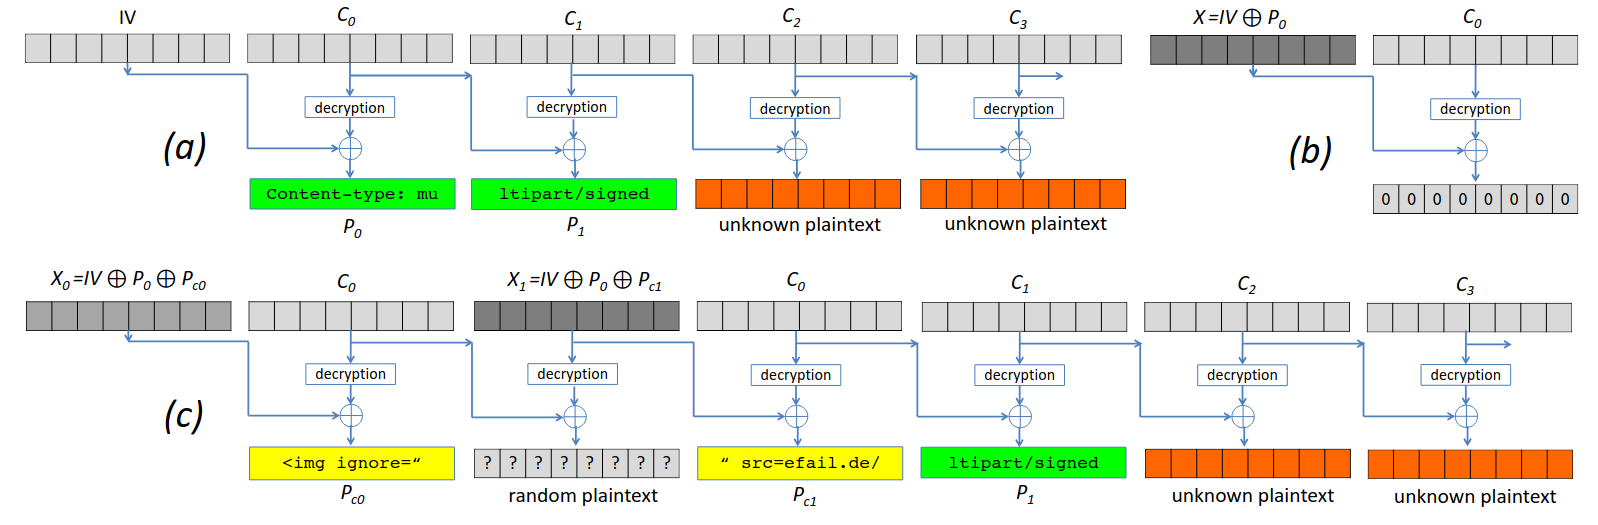
\includegraphics[width=\textwidth]{img/efail.png}
    \par}

    Protocolli crittografici: \textbf{s/MIME} + \textbf{OpenPGP} (\textbf{AES-CBC}), vettore di attacco: \textbf{\textit{Man in the middle}}. L'attaccante esponeva un servizio web che corrispondeva a \textbf{http://efail.de/ltipart/signed} e riuscia a leggere la mail in chiaro all'interno della richiesta.
\end{flushleft}

% PAGINA VUOTA
%\clearpage\null\thispagestyle{empty}\clearpage
%\appendix
%\appendixpage
%\addappheadtotoc

%\clearpage\null\thispagestyle{empty}\clearpage


%\listoffigures


\begin{flushleft}
\bibliographystyle{plain}
\bibliography{sections/references} 
\end{flushleft}

\end{document}
